%
% Capítulo 2
%
\chapter{Trabalho Relacionado} \label{cap:trabrelacionado}
Neste capítulo vamos abordar sistemas relacionados com o nosso trabalho e alguns sistemas semelhantes ao que vamos desenvolver.\\
A elaboração deste projeto envolve vários componentes externos, pelo que será importante analisar os vários componentes com os quais vamos interagir.\\
Na secção \ref{sec:cont} vamos analisar os contadores de água com os quais o nosso sistema vai interagir. Nas secções \ref{sec:appsmas} e \ref{sec:telemetria} vamos abordar algumas soluções já existentes no mercado com funções semelhantes à do sistema que vamos desenvolver.

\section{Contadores de Água} \label{sec:cont}
Para a realização deste projeto é importante analisar os dispositivos contadores de água, dado que o nosso sistema vai interagir com eles, nomeadamente, obtendo a sua medição.
Existem vários tipos de contadores de água, diferindo na aparência, no contexto que devem ser utilizados (residencial, comercial, industrial) ou na forma como registam a quantidade de água que passa por eles. Para este projeto, nós vamos interagir apenas com o dispositivo indicador, que é o local do contador que indica a leitura de água e o seu número de série.
A figura \ref{fig:contador} contém uma imagem de um contador, onde podemos observar no retângulo 1 ( a verde) a medição do contador e no retângulo 2 (a azul) o ano e número de série do contador.

\begin{figure}[h!]
\begin{center}
\resizebox{80mm}{!}{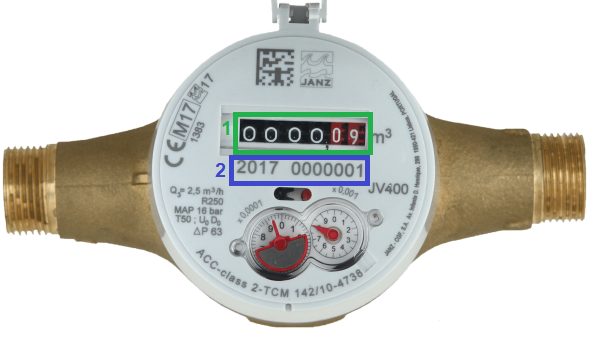
\includegraphics{diagramas/contador.png}}
\caption{Dispositivo indicador do contador de água.}
\label{fig:contador}
\end{center}
\end{figure}


Existem sistemas com funções e finalidades próximas ou até iguais ao sistema que vamos conceber. Deveremos analisar as várias funções destes sistemas, porém também as suas falhas e funcionalidades que deveriam ter sido implementadas, para que no nosso sistema possamos colmatar essas situações e oferecer uma solução mais competente e vantajosa.

\section{Aplicação para Dispositivo Móvel} \label{sec:appsmas}
Os Serviços Municipalizados de Água e Saneamento de Almada e de Sintra já possuem, respetivamente, aplicações para \textit{smartphone} \cite{smas:almada} e websites \cite{smas:sintra} para as diferentes zonas em que operam. Estas plataformas permitem a gestão do contrato, consulta de contas, faturas e consumos, ativação de pagamento por débito direto, alteração de dados pessoais e a comunicação de leituras.

\section{Sistemas de Telemetria} \label{sec:telemetria}
Existem, aplicados a esta área, sistemas de telemetria, ou seja, sistemas que efetuam a medição e comunicação das leituras. Alguns destes sistemas vêm incorporados no aparelho contador, existindo também outros que são um dispositivo separado \cite{janz:impji}. Porém, neste último caso, o contador de água tem de ser construído com características próprias que lhe permitam comunicar com estes dispositivos.
